\section{Results}\label{sec:results}
This section reports the outcomes of the tests defined in
Section~\ref{sec:evaluation}, in the order of the research questions. Results
from synthetic experiments and full-horizon local \textit{Laya} case runs
are distinguished because they support different kinds of claim.

\subsection{Mechanism Checks (RQ1, RQ2)}\label{sec:res-mechanisms}
The first experiment checks the game-analysis tool on a small coordination
game. A founder chooses whether to fund an independent review, and a
liquidity partner chooses whether to commit funds to escrow or wait.
Table~\ref{tab:game} gives both players' assumed utilities, which are
preference points rather than cash. The tool finds exactly two pure Nash
equilibria, review/commit and skip/wait: in each, either player would lose by
changing its action alone. If the founder believes the partner commits with
probability $0.4$, Eq.~\eqref{eq:eu} gives an expected utility of
$0.4\times6+0.6\times(-2)=1.2$ for review and $0.4\times2+0.6\times0=0.8$ for
skipping, so skipping has a regret of $0.4$ by Eq.~\eqref{eq:regret}. The tool
returns these values as exact fractions ($6/5$, $4/5$, and $2/5$).

\begin{table}[t]
\caption{Experiment 1 utilities: (founder, partner).}
\label{tab:game}
\centering\footnotesize
\begin{tabular}{@{}lcc@{}}
\toprule & Partner commits & Partner waits \\
\midrule
Founder funds review & $(6,5)$ & $(-2,1)$ \\
Founder skips review & $(2,-4)$ & $(0,0)$ \\
\bottomrule
\end{tabular}
\end{table}

The second experiment applies Eq.~\eqref{eq:bayes} twice. Two hypotheses,
that attention to the token persists or fades, start with priors $0.4$ and
$0.6$. A first signal has likelihood $0.75$ if attention persists and $0.25$
if it fades, which raises the persistence posterior to $2/3$. A second signal
with likelihoods $0.6$ and $0.3$, assumed independent of the first given the
hypothesis, raises it to $4/5$. Both match the hand calculation. The
independence assumption is what allows the two likelihoods to be multiplied;
correlated signals would need a joint likelihood to avoid counting the same
information twice.

The third experiment follows two builders, each with 100 cents, through two
rounds of a world with one bounded readiness metric
(Table~\ref{tab:timing}). A scheduled event raises readiness from 1 to 2
before the first observations. Both builders then spend 60 cents on an
action worth 6 points each; the effects sum to 14 and Eq.~\eqref{eq:settlement}
clips the result to the upper bound of 10. A second scheduled event lowers it
to 9 before the next observations, and with only 40 cents left, building is
no longer affordable, so both builders wait. Remaining cash plus spending is
$40+40+120=200$ cents, as Eq.~\eqref{eq:conservation} requires, and replay
reproduces every state exactly. The build-then-wait policy is imposed, so
this tests execution rather than any model's choices.

\begin{table}[t]
\caption{Experiment 3: state over time. Cash is in cents.}
\label{tab:timing}
\centering\footnotesize
\begin{tabular}{@{}lrrrr@{}}
\toprule Stage & Readiness & Alice & Bob & Spent \\
\midrule
Initialization & 1 & 100 & 100 & 0 \\
Round-one observation & 2 & 100 & 100 & 0 \\
Round-one settlement & 10 & 40 & 40 & 120 \\
Round-two observation & 9 & 40 & 40 & 120 \\
Terminal state & 9 & 40 & 40 & 120 \\
\bottomrule
\end{tabular}
\end{table}

The fourth experiment checks the scoring formulas. Two synthetic training
outcomes give a baseline positive rate of $0.5$. On two later cases with
outcomes $(0,1)$, supplied forecasts $(0.25,0.75)$ score a Brier value of
$0.0625$ and a log loss of $0.287682$ by Eqs.~\eqref{eq:brier}
and~\eqref{eq:logloss}, against $0.25$ and $0.693147$ for the constant
baseline. Two invented cases confirm the formulas, not any forecasting
skill.

Experiments 5 and 6 turn from arithmetic to RQ2, isolating one mechanism at a
time. In Experiment 5, Alice builds in round one and publishes a message; Bob
joins in round two only if he receives it, and a declared joint rule adds
three readiness points when Alice waits while Bob joins. Switching delivery
and the joint rule on and off (Table~\ref{tab:ablation}) separates the two
effects. Removing only the joint rule leaves Bob's choice unchanged but lowers
final readiness from 6 to 3. Removing delivery changes Bob's choice to waiting,
so the joint rule never activates and readiness stays at 1. One mechanism
therefore changes what an actor does, and the other changes what that
action is worth. All four runs replay exactly and conserve the 200 cents of
starting cash.

\begin{table}[t]
\caption{Experiment 5: delivery and joint-rule ablation. Cost and cash are in
cents; starting cash is 200 in every condition.}
\label{tab:ablation}
\centering\footnotesize
\begin{tabular}{@{}llrrr@{}}
\toprule Delivery & Joint rule & Readiness & Cost & Cash left \\
\midrule
On & On & 6 & 50 & 150 \\
On & Off & 3 & 50 & 150 \\
Off & On & 1 & 20 & 180 \\
Off & Off & 1 & 20 & 180 \\
\bottomrule
\end{tabular}
\end{table}

Experiment 6 asks whether an actor's behavior follows its numeric
preferences or its persona text. An eight-role world is run with the
deterministic offline rule, which picks the action with the greatest
immediate utility change. Under the declared weights, the
participation-oriented role joins and the risk-sensitive role waits. Changing
only the former's risk weight from $-500$ to $-5{,}000$ turns its joining
value from $8{,}500$ to $-5{,}000$ utility points, and it waits instead; final
participation falls from 44 to 34, risk from 24 to 18, and total spending from
120{,}000 to 110{,}000 cents. Rewriting every role's motivation and goal to
emphasize caution, while keeping the weights fixed, changes nothing at all.
In this baseline, then, the prose describes an actor but the weights
determine its behavior. Whether \textit{Laya} also follows the
weights rather than the prose is a separate question that these experiments
do not answer.

Beyond the six experiments, the engine's automated suite of \rev{1{,}904 passed
tests (with two optional-dependency skips) verified} the code used for this
paper, covering, among others, the market maker, \rev{the collateralized
lending ledger,} checkpoint recovery, actor inference adapters, and the MCP server. The six experiments' outputs are regenerated with network
access disabled and match the saved records byte for byte.

\subsection{MACRON Case Study (RQ3)}\label{sec:res-macron}
\begin{revised}
Moving from mechanism checks to full-horizon execution, all 24 local
\textit{Laya} paths reached hour 336, covering all 8{,}064 planned path-hours.
They record 8{,}754 decision points and 136{,}841 local requests with no per-call
API fee (Table~\ref{tab:macron-laya}). All paths were independently replayed
from packages, seeds, and saved choices. These results demonstrate execution
coverage under the selected world rules, not predictive accuracy.

Across the saved receipts, cumulative inference elapsed time is
146{,}873.669 seconds (about 40.8 hours). This sums per-call elapsed times
across concurrent workers; it is neither end-to-end wall-clock duration nor
CPU core-hours. Every receipt identifies local \textit{Laya} transport and
records zero API fee. Hardware, electricity, setup, data access, and other
execution overhead remain outside that fee measurement.
\end{revised}

\begin{table}[t]
\caption{\rev{Full-horizon \textit{MACRON} paths decided by \textit{Laya} from
hour 0. Each regime has 12 paths; cash amounts are simulated U.S.\ dollars, and
all rejections are slippage rejections.}}
\label{tab:macron-laya}
\centering\footnotesize\color{revisedred}
\renewcommand{\arraystretch}{1.1}
\begin{tabular}{@{}lrr@{}}
\toprule
Measure & \textit{BULL} & \textit{BEAR} \\
\midrule
Last hour reached (all paths) & 336 & 336 \\
Completed path-hours (of 4{,}032) & 4{,}032 & 4{,}032 \\
Replay-verified decision points & 4{,}381 & 4{,}373 \\
Local \textit{Laya} requests & 68{,}508 & 68{,}333 \\
Filled buys & 13{,}913 & 13{,}433 \\
Filled sells & 11{,}459 & 11{,}446 \\
Rejected trades & 5{,}894 & 5{,}456 \\
Traded cash (\$) & 8{,}493{,}778 & 8{,}282{,}843 \\
\bottomrule
\end{tabular}
\end{table}
\begin{revised}
Within those paths, the engine filled 25{,}372 trades in \textit{BULL} and
24{,}879 in \textit{BEAR}. It recorded 11{,}350 slippage rejections in total
instead of settling orders outside the permitted limits. The terminal state
is the end of observation; it does not by itself establish termination of the
hypothetical project.
\end{revised}

\subsection{Comparison with \textit{MiroFish} (RQ4)}\label{sec:res-mirofish}
With the same brief, \textit{MiroFish} and \textit{Boyun} produced records
of a different kind, and Table~\ref{tab:mirofish} places them side by side.
Both \textit{MiroFish} regimes and all 24 local \textit{Boyun} paths
completed the planned 336 hours. Over those rounds, its
sixteen personas wrote 537 original posts and 396 quote posts under
\textit{BULL}, against 371 and 206 under \textit{BEAR}, and chose to do
nothing 819 and 859 times. The posts are written in each persona's own voice and
respond to one another; a promoter, for example, quotes the founder's launch
post to pitch paid attention as the real driver of demand.
\textit{Boyun}'s messages, by contrast, are pre-written texts attached to
actions, so its social layer is far less expressive.

\begin{table}[t]
\caption{\textit{MACRON} under the original \textit{MiroFish} and under
\textit{Boyun} (full-horizon local \textit{Laya} paths), as \textit{BULL}\,/\,\textit{BEAR}.
Counts are recomputed from each system's saved databases.}
\label{tab:mirofish}
\centering\footnotesize\color{revisedred}
\renewcommand{\arraystretch}{1.1}
\begin{tabularx}{\columnwidth}{@{}>{\raggedright\arraybackslash}p{0.3\columnwidth}YY@{}}
\toprule
Measure & \textit{MiroFish} & \textit{Boyun} \\
\midrule
Actor model & \textit{Gemini} 3.5 Flash-Lite & \textit{Laya} \\
Paths per regime & 1 social path & 12 plan paths \\
Hours completed & 336 / 336 & 336 / 336 \\
Original posts & 537 / 371 & -- \\
Quote posts & 396 / 206 & -- \\
Likes and reposts & 153 / 154 & -- \\
Do-nothing actions & 819 / 859 & -- \\
Filled trades & not modeled & 25{,}372 / 24{,}879 \\
Rejected trades & not modeled & 5{,}894 / 5{,}456 \\
Settled cash and tokens & not modeled & integer ledgers \\
Matched policy pairs & none & 6 / 6 \\
Replay of decisions & not available & 4{,}381 / 4{,}373 points \\
Confirmed model requests & 1{,}911 / 1{,}499 & 136{,}841 local calls \\
Model cost & free quota & zero API fee \\
Reporting focus & social discourse & settled finances and policy comparison \\
\bottomrule
\end{tabularx}
\end{table}

The financial side of the comparison runs the other way. \textit{MiroFish}
models no orders, balances, or pool, so a post enthusiastic about buying
changes no price and no founder's cash, and the founder's question, how much
money each plan keeps, cannot be answered from its output. \textit{Boyun}
settles every trade, records why rejected trades failed, compares plans at
matched times, and replays every saved decision. \textit{MiroFish}'s original
random state was not checkpointed and had to be reseeded during recovery,
so its runs cannot be reproduced decision by decision.

\begin{revised}
The output distinction also shapes reporting. The saved \textit{MiroFish}
reports discuss sentiment, stakeholder behavior, and risks in prose, whereas
\textit{Boyun}'s case analysis uses settled trades, recorded failures, and
policy differences. Neither output establishes what will happen in a real
launch. Different models, activation rules, and recovery procedures prevent
interpreting this comparison as a general performance ranking.
\end{revised}

\subsection{Local Actor Behavior (RQ5)}\label{sec:res-laya}
\begin{figure}[t]
\centering
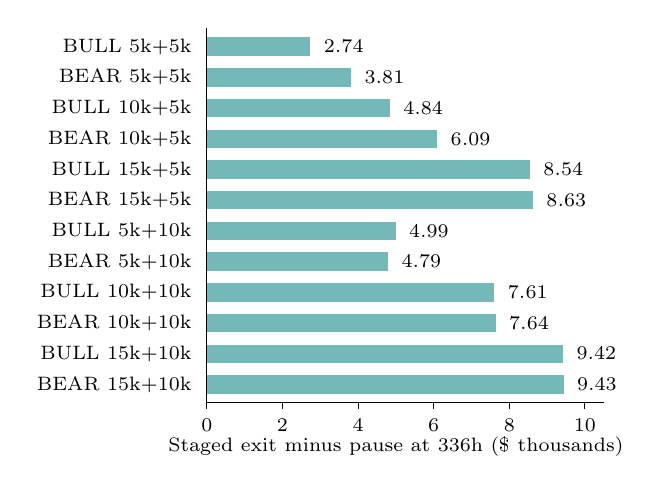
\begin{tikzpicture}[x=0.48cm,y=0.39cm,font=\scriptsize]
\foreach \lab/\val [count=\i] in {
 BULL 5k+5k/2.73637,
 BEAR 5k+5k/3.81432,
 BULL 10k+5k/4.83896,
 BEAR 10k+5k/6.09226,
 BULL 15k+5k/8.54469,
 BEAR 15k+5k/8.62541,
 BULL 5k+10k/4.99001,
 BEAR 5k+10k/4.79270,
 BULL 10k+10k/7.60652,
 BEAR 10k+10k/7.63833,
 BULL 15k+10k/9.42026,
 BEAR 15k+10k/9.43499}{
 \fill[teal!55] (0,-\i+0.3) rectangle (\val,-\i-0.3);
 \node[anchor=east] at (-0.15,-\i) {\lab};
 \node[anchor=west] at (\val+0.1,-\i) {\pgfmathprintnumber[fixed,precision=2]{\val}};
}
\draw (0,-0.4)--(0,-12.6)--(10.5,-12.6);
\foreach \v in {0,2,4,6,8,10} {\draw (\v,-12.6)--(\v,-12.8) node[below] {\v};}
\node[below] at (5,-13.4) {Staged exit minus pause at 336h (\$ thousands)};
\end{tikzpicture}
\caption{\rev{Cash difference $D_p$ for all 12 local \textit{Laya} plan pairs
at the common terminal hour 336. Labels give regime, founder position budget,
and upfront cost, in thousands of dollars. Unsold inventory is excluded;
therefore these bars do not rank total wealth.}}
\label{fig:matched-laya}
\end{figure}

\begin{revised}
Beyond coverage, the completed matrix exposes limits of the actor model.
\textit{Laya} produced similar traded cash across the two regimes:
\$8{,}493{,}778 in \textit{BULL} and \$8{,}282{,}843 in \textit{BEAR}, a gap
of approximately 2.5\%. Across 136{,}841 multi-option requests, its mean top
score was 0.42. Near-uniform option scores, combined with the engine's sampling
rule, are consistent with heavy two-way turnover and weak regime separation.
The recorded rejection count is about 1.30 per decision point. These
observations motivate behavioral validation rather than a market forecast.

Despite weak regime separation, staged exit held between \$2{,}736.37 and
\$9{,}434.99 more realized cash than pause in all 12 pairs at hour 336
(Figure~\ref{fig:matched-laya}). Founder purchases and exit tranches follow
explicit policy rules, so this cash comparison is not evidence that the actor
model discovered a superior strategy. In all six \$10{,}000-upfront pairs,
upfront spending alone meets the \$10{,}000 loss-budget alert at launch.

Including unsold inventory changes the interpretation. At hour 336 its pool
quote is between \$4{,}278 and \$11{,}805 under pause. Adding that quote to cash
puts pause ahead by \$464--\$3{,}260 in the six \$5{,}000-upfront pairs; staged
exit remains \$256--\$843 ahead in the six \$10{,}000-upfront pairs. A pool
quote is not guaranteed executable proceeds. The comparison must therefore
show realized cash and retained inventory separately.
\end{revised}

\subsection{NEAR Lending Case Study (RQ6)}\label{sec:res-lending}
\begin{revised}
Apart from sampled token trading, four local \textit{Laya} lending worlds
complete 90 days each (2{,}160 hours), with decisions selected by argmax.
Their event journals support exact ledger replay. Table~\ref{tab:lending}
summarizes only those four worlds; hosted and mixed-model runs are excluded.
\end{revised}

\begin{table}[t]
\caption{Local \textit{Laya} lending worlds after 90 days. Protocol share is 15\% of borrower
interest, collected plus still owed. Campaign spending was \$20{,}000 in each local world. ``Borrowed'' counts decisions in which borrowing was offered
and chosen.}
\label{tab:lending}
\centering\footnotesize\color{revisedred}
\renewcommand{\arraystretch}{1.1}\setlength{\tabcolsep}{3pt}
\begin{tabular}{@{}lrrrrr@{}}
\toprule
World & Lent, day 30 & Peak use & Liquid. & Protocol \$ & Borrowed \\
\midrule
C-P50-R2-L & \$300K & 15.6\% & 1 & 361 & 54/54 \\
C-P100-R2-L & \$500K & 25.8\% & 12 & 703 & 292/295 \\
C-P100-R8-L & \$500K & 25.8\% & 13 & 1{,}802 & 258/260 \\
B-P100-R8-L & \$374K & 19.5\% & 20 & 1{,}077 & 431/433 \\
\bottomrule
\end{tabular}
\end{table}

First, the observed borrowing ceilings reflect explicit caps, while whether
actors reach them depends on their choices. In C-P50-R2-L each of the six borrowing
accounts reached its \$50{,}000 cap by day 30, and once that cap was raised,
both \textit{Laya} choppy worlds reached the \$500{,}000 aggregate cap by the
same day. With about \$2{,}000{,}000 supplied, utilization could not exceed
about 25\%. Under Eq.~\eqref{eq:rate}, suppliers therefore earned about 1\% a
year under curve R2 and 2.4\% under R8, against \textit{RHEA}'s 9.88\%;
matching \textit{RHEA} at 25\% utilization would require a borrow rate near
46\%. Second, the risk rules left no bad debt in any world, and the loss
reserve was never used. On the bear path, hourly closes fell 68\% and twenty
liquidations repaid \$302{,}000 without loss.

That second result carries two conditions. It depends on the assumed
liquidators' cash and exit depth, which were not measured, and on the
oracle's hourly sampling. On 10 October 2025 NEAR briefly traded 40\% below
the choppy window's opening price but closed that hour about 9\% lower, so the
deepest fall the ledger saw on that path was 31\%, and its liquidations came
on days 60--61, 67, and 80--85. Liquidations during such intrahour moves remain
untested.

\begin{revised}
The behavioral observations require a different interpretation.
Borrowing was selected in 258 of 260 offered decisions under curve R8 and
292 of 295 under curve R2 in the choppy worlds. This near-saturation persists
despite materially different rates and should not be read as measured demand.
Partner acceptance, supply retention, and campaign reach also depend on
uncalibrated model choices and synthetic balances. Real borrower intentions,
observed conversion, and multiple seeds are needed before extrapolating those
behaviors.
\end{revised}

Within these four worlds, the launch's modeled economics are thin. Over 90 days, the
protocol's share of interest ranged from \$361 to \$1{,}802 in the
\textit{Laya} worlds, against \$20{,}000 spent on the campaign.
